\section{Introduction}

As Large Language Models (LLMs) achieve strong performance on complex reasoning tasks~\citep{wei2022chain,jaech2024openai,ICLR2024_d53538ba}, modern reasoning alignment often assumes that each query is well-posed and has a determinate answer~\citep{chen2025towards}. Under this assumption, models can be rewarded for reaching the verified answer and penalized or left unrewarded otherwise~\citep{guo2025deepseek}. Yet many queries violate this premise: they may omit necessary information or contain contradictory constraints, so no determinate answer exists under the requested response format. Prior work on confidence calibration~\citep{xiong2023can,yoon2025reasoning,fisch2022calibrated,chen2025aware} and capability boundaries~\citep{NEURIPS2024_62ab1c2c,zhang2025self,kalai2025languagemodelshallucinate} mainly examines when models should abstain from unproductive reasoning on otherwise valid tasks; TruthRL~\citep{wei2025truthrl} further encourages refusal under uncertainty via a ternary reward.

\begin{figure}[t]
    \centering
    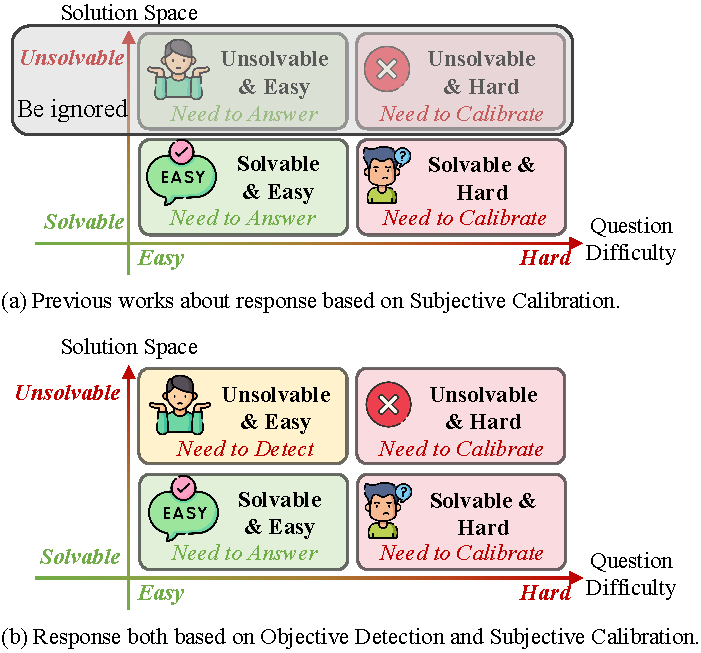
\includegraphics[width=\linewidth]{figures/intro_2.pdf}
    \caption{Comparison of alignment paradigms. We treat the solution space (solvable vs. unsolvable) and question difficulty (easy vs. hard) as orthogonal dimensions, requiring models to \textbf{detect input-side defects}, \textbf{solve feasible tasks}, and \textbf{calibrate refusal} on hard but solvable problems.}
    \label{fig:intro_quadrant}
\end{figure}

This model-side focus overlooks flawed queries whose specifications make a determinate answer impossible, such as missing information or logical contradictions. These cases are not merely difficult: the requested answer is not well-defined. We call the resulting distinction the \textit{solvability boundary}, and treat \textit{Solution Space} (solvable vs. unsolvable) and \textit{Question Difficulty} (easy vs. hard) as orthogonal dimensions (Figure~\ref{fig:intro_quadrant}). A reliable system must therefore decouple three behaviors: solving feasible tasks, detecting unsolvable inputs, and calibrating refusal when a solvable problem exceeds current capacity. Current LLMs often blur this boundary, leading to a ``refusal dilemma'': they hallucinate answers to invalid queries, or over-refuse valid but difficult problems.



To learn this boundary, we introduce \textbf{UnsolvableQA}, a benchmark suite of paired solvable and unsolvable instances across logic and mathematics, with science-domain diagnostic and OOD extensions, built via \textit{Reverse Construction} with constraint conflicts and missing-information cases for diagnostic analysis. Verifier-backed structured domains use deterministic solvers; math instances undergo cross-model verification and human auditing. We further propose \textbf{UnsolvableRL} (GRPO~\citep{shao2024deepseekmath}), optimizing (1) unsolvability detection, (2) a false-unsolvability penalty, and (3) dynamic capability calibration when empirical accuracy falls below a target threshold.

Empirical results show solvability boundary learning acts as an effective reasoning regularizer. UnsolvableRL improves the unsolvable detection rate of Qwen3-4B from 38.8\% to 87.5\%, while simultaneously increasing solvable problem accuracy from 43.4\% to 69.4\%. On Llama3-8B, mean score improves from 25.2\% to 55.1\% (+29.9\%; 119\% relative improvement), with OOD gains on GPQA (+12.0\%) and MMLU-Pro (+4.5\%). Diagnostic tuning enables MI/CC attribution and IN3 clarification transfer (Detail Recovery 47.8\%$\rightarrow$60.7\% for Llama3-8B). Ablations reveal \textit{Capability Collapse} when penalties are applied without unsolvable data, whereas our joint framework turns them into a rigor regularizer.

Overall, our main contributions are:
\begin{itemize}[leftmargin=16pt, itemsep=0pt, topsep=0pt]
    \item We construct \textbf{UnsolvableQA}, a verifier-backed benchmark suite spanning logic and math, with science-domain diagnostic/OOD evaluation, built via Reverse Construction with deterministic checks and audited math verification.
    \item We propose \textbf{UnsolvableRL} for \textit{solvability boundary learning}, decoupling reasoning on solvable tasks, unsolvability detection, and capability-calibrated refusal in a unified alignment framework.
    \item We show that learning solvability boundaries improves both solvable accuracy and unsolvability detection, prevents capability collapse under refusal penalties, and extends beyond binary detection to defect diagnosis and zero-shot clarification transfer.
\end{itemize}
